
\begin{tcolorbox}[title=Quick Start,colback=blue!1,colframe=blue!30!black,breakable]
Install the required Python packages:
%
\begin{lstlisting}[language=bash,basicstyle=\ttfamily,frame=none,numbers=none]
    pip install qmcpy numpy matplotlib
\end{lstlisting}

Generate 16 paths on $\lbrack 0,1\rbrack$ with QMCPy's sampler  ($S_0=1$, $\mu=0.05$, $\sigma^2=0.2$) and plot five:
%
\lstinputlisting[
    style=Python,
    frame=none,
    numbers=none,
    label={lst:quickstart}
]{GBM/code/quickstart.py}
\end{tcolorbox}


\subsection{Introduction}

In this blog, we demonstrate how to simulate and analyze a geometric Brownian motion (GBM) process using QMCPy in Python.
GBM is widely used in finance to model stock prices and other assets. 
We will walk through key code snippets, plots, and insights. The numerical results can be reproduced using the Jupyter notebook available at \href{gbm\_demo.ipynb}{\url{https://github.com/QMCSoftware/QMCSoftware/blob/master/demos/gbm\_demo.ipynb}}.

GBM is a continuous stochastic process in which the natural logarithm of its values follows a Brownian motion (BM) $[1]$.
Mathematically, it can be defined as follows:
\begin{equation}
S_t = S_0 \, e^{\bigl(\mu - \tfrac{\sigma^2}{2}\bigr)  t + \sigma W_t}, \label{gbm}
\end{equation}
where
\begin{itemize}
\item $S_0$ is the initial value, 
\item $\mu$ is a drift coefficient
\item $\sigma$ is the volatility (note: QMCPy uses diffusion = $\sigma^2$)
\item $W_t$ is a (standard) BM.
\end{itemize}

At any time $0 < t \le T$, where $0$ and $T$ represent the beginning and end time of the process, $S_t$ follows a log-normal distribution with expected value and variance as follows (see Section 3.2 in $[1]$):
\begin{itemize}
\item
 $E[S_t] = S_0 e^{\mu t}$
\item $\text{Var}[S_t] = S_0^2 e^{2\mu t}(e^{\sigma^2 t} - 1)$
\item   $  
    \text{Cov}(S_{t_i}, S_{t_j}) = S_0^2 e^{\mu(t_i + t_j)} \left(e^{\sigma^2 \min(t_i, t_j)} - 1\right).$
\end{itemize}

GBM is commonly used to model stock prices driving option payoffs in derivatives pricing $[4, 5]$. 

\subsection{GBM Objects in QMCPy}

GBM in QMCPy inherits from BrownianMotion class $[2, 3]$. 
We can create a simple GBM instance and generate sample paths to see the class in action; see Listing~\ref{lst:gbm_qmcpy2}:

\lstinputlisting[
    style=Python,
    caption={Generating 4 GBM sample paths evaluated at 2 time points using QMCPy.},
    label={lst:gbm_qmcpy2}
]{GBM/code/gbm_qmcpy.py}

The output shows 4 sample paths evaluated at 2 time points, yielding a $(4 \times 2)$ array where rows represent paths and columns represent time steps:
\[
\left[
\begin{array}{@{} S[table-format=1.8] S[table-format=1.8] @{}}
\num{0.72608046} & \num{0.70071241} \\
\num{0.38739775} & \num{0.07432173} \\
\num{0.81262942} & \num{1.66867239} \\
\num{0.619371} & \num{0.31898397}
\end{array}
\right].
\]

\subsection{Log-Normality Property}

The log-normal property is fundamental in financial modeling because it ensures asset prices remain strictly positive (as required in reality) while allowing for unlimited upside potential. This property makes GBM the cornerstone of the Black-Scholes model and many derivative pricing frameworks.

To validate theoretical properties, we generate $2^{12} = 4096$ paths over 5 time steps and compare empirical moments with theoretical values.  Note that the theoretical values match the last values captured in \texttt{qp\_gbm.mean\_gbm} and \texttt{qp\_gbm.covariance\_gbm} for the final time point. The results are shown in Table~\ref{tab1}.

\lstinputlisting[
    style=Python,
    caption={Generating and validating GBM sample moments.},
    label={lst:gbm-validation}
]{GBM/code/gbm_moments_validation.py} 

\begin{table}[tbp]
\centering
\caption{Theoretical vs Empirical Validation of GBM Properties.}
\begin{tabular}{ll}
\hline
\textbf{Statistic} & \textbf{Value} \\
\hline
Sample Mean & 105.127 (Theoretical: 105.127) \\
Sample Variance & 449.776 (Theoretical: 451.029) \\
\hline
Time Vector & [0.2,\; 0.4,\; 0.6,\; 0.8,\; 1.0] \\
Drift ($\mu$) & 0.05 \\
Diffusion ($\sigma^2$) & 0.040\\
Mean  & [101.005,\; 102.020,\; 103.045,\; 104.081,\; 105.127] \\
Decomposition Type & PCA \\
\hline
Covariance Matrix & 
\(
\left[\begin{array}{rrrrr}
81.943 &  82.767 &  83.599 &  84.439 &  85.288 \\
82.767 & 167.869 & 169.556 & 171.260 & 172.981 \\
83.599 & 169.556 & 257.923 & 260.516 & 263.134 \\
84.439 & 171.260 & 260.516 & 352.258 & 355.798 \\
85.288 & 172.981 & 263.134 & 355.798 & 451.029
\end{array}\right]
\)
\\
\hline
\end{tabular}
\label{tab1}
\end{table}

\subsection{GBM vs BM}

Below we compare BM and GBM using the same parameters: $\texttt{drift} = 0$, $\texttt{diffusion} = 1$, $\texttt{initial\_value} = 1$.
The driftless BM paths should fluctuate symmetrically around the initial value ($y = 1$) and can take negative values, while those of the GBM remain strictly positive. We generate these samples in Listing~\ref{lst:gbm_qmcpy3}.

\lstinputlisting[
    style=Python,
    caption={Generate 16 BM and 16 GBM sample paths.},
    label={lst:gbm_qmcpy3}
]{GBM/code/bm_gbm_16.py}

Next, we demonstrate how easily one can swap samplers or change parameters in QMCPy.  For example, to model a stock price
with initial value $S_0=50$, drift $\mu=0.1$, and volatility $\sigma=\sqrt{0.2}$ over a 5‐year horizon using IID sampling; see Listing~\ref{lst:gbm_iid_32}.

\lstinputlisting[
    style=Python,
    caption={Generate 32 GBM sample paths with IID sampling.},
    label={lst:gbm_iid_32}
]{GBM/code/gbm_iid_32.py}

Or, to use a low‐discrepancy lattice sampler with the same parameters (Listing~\ref{lst:gbm_lattice_32}):
\lstinputlisting[
    style=Python,
    caption={Generate 32 GBM sample paths with lattice sampling.},
    label={lst:gbm_lattice_32}
]{GBM/code/gbm_lattice_32.py}

%Now, let's define a utility function that will help us visualize BM or GBM paths with different samplers and parameters (Listing~\ref{lst:plot-paths}). 
The generated sample paths are plotted in Figure~\ref{fig:bm_gbm_paths}. Subplots~(\subref{fig:bm_iid}), (\subref{fig:gbm_iid}), (\subref{fig:bm_lattice}), and (\subref{fig:gbm_lattice}) show, respectively: 

\begin{itemize}
    \item BM with lattice sampler ($T=1$, $S_0=1$, $\mu=0$, $\sigma^2=1$, 16 paths)
    \item GBM with lattice sampler ($T=1$, $S_0=1$, $\mu=0$, $\sigma^2=1$, 16 paths)
    \item GBM with IID sampler ($T=5$, $S_0=50$, $\mu=0.1$, $\sigma^2=0.2$, 32 paths)
    \item GBM with lattice sampler ($T=5$, $S_0=50$, $\mu=0.1$, $\sigma^2=0.2$, 32 paths).
\end{itemize}

\begin{comment}
\lstinputlisting[
    style=Python,
    caption={Function to plot BM and GBM sample paths.},
    label={lst:plot-paths}
]{GBM/code/plot_paths.py}
\end{comment}

\begin{figure}[tbp]
\centering
\begin{subfigure}[t]{0.49\textwidth}
\centering
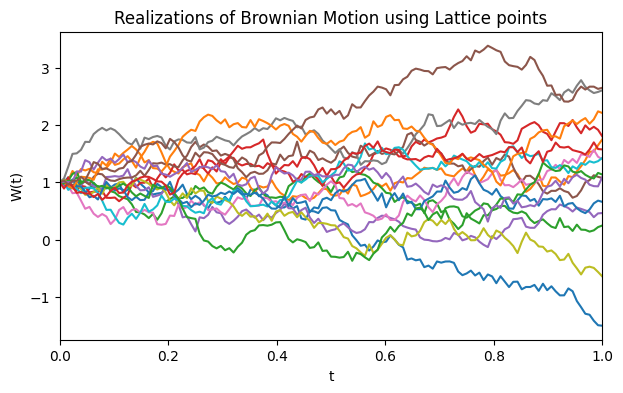
\includegraphics[width=\textwidth]{GBM/images//figure_1.png}
\caption{}
\label{fig:bm_iid}
\end{subfigure}
\begin{subfigure}[t]{0.49\textwidth}
\centering
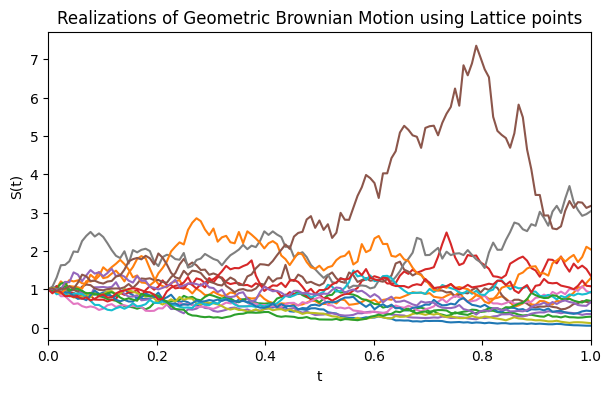
\includegraphics[width=\textwidth]{GBM/images//figure_2.png}
\caption{}
\label{fig:gbm_iid}
\end{subfigure}
\begin{subfigure}[b]{0.49\textwidth}
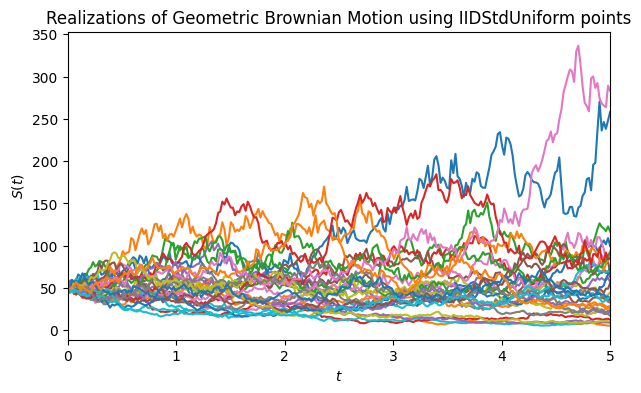
\includegraphics[width=\textwidth]{GBM/images//figure_3.png}
\caption{}
\label{fig:bm_lattice}
\end{subfigure}
\hfill
\begin{subfigure}[b]{0.49\textwidth}
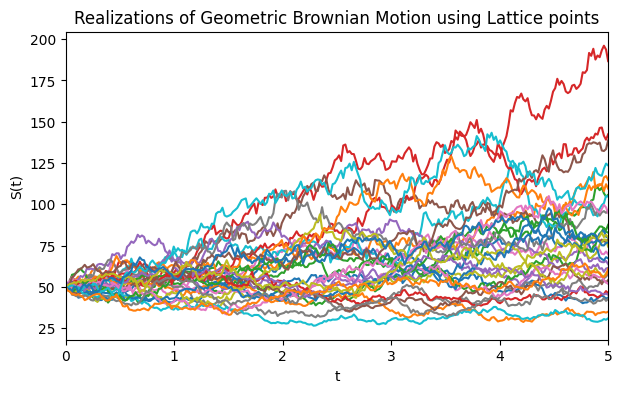
\includegraphics[width=\textwidth]{GBM/images//figure_4.png}
\caption{}
\label{fig:gbm_lattice}
\end{subfigure}
\caption{Comparison of sample paths for BM and GBM using different samplers.}
\label{fig:bm_gbm_paths}
\end{figure}

\subsection{QuantLib vs QMCPy Comparison}

In this section, we compare QMCPy's GeometricBrownianMotion implementation with the industry-standard QuantLib library [6] to validate its accuracy and performance. %We use Listing~\ref{lst:quantlib} to generate the QuantLib paths.
The numerical results are summarized in Table~\ref{tab2}. 

Both libraries produce statistically equivalent GBM simulations that match theoretical values. QMCPy typically runs 1.5 to 2 times faster due to vectorized operations, lazy loading, and optimized memory management. More importantly, it demonstrates superior numerical accuracy (lower mean absolute errors) with Sobol, lattice and Halton samplers, making it excellent for research and high-performance applications. QuantLib remains the industry standard for production systems that require comprehensive support for financial modeling and risk management.

\lstinputlisting[
    style=Python,
    caption={Function to generate GBM paths with QuantLib.},
    label={lst:quantlib}
]{GBM/code/quantlib_util.py}

\begin{table}[tbp]\centering
\caption{GBM Final Value Statistics and Performance Comparison}
\label{tab2}
\begin{tabular}{ll@{\hspace{0.4em}}r@{\hspace{0.4em}}r@{\hspace{0.4em}}r@{\hspace{0.4em}}r@{\hspace{0.4em}}r@{\hspace{0.4em}}r@{\hspace{0.4em}}r}
\toprule
Method & Sampler & Mean & Std Dev & Mean  & Std Dev  & Mean Time (s)  & Std Dev (s) & Speedup \\
 &  &  &   &  Error &  Error &   & &  \\
\midrule
QuantLib & IIDStdUniform & 105.3313 & 21.4671 & 0.2042 & 0.2296 & 0.8122 & 0.0000 & - \\
QMCPy & IIDStdUniform & 105.1443 & 21.3848 & 0.0172 & 0.1474 & 0.5217 & 0.0000 & 1.5569 \\
QuantLib & Sobol & 105.0905 & 21.0145 & 0.0366 & 0.2229 & 0.8852 & 0.0000 & - \\
QMCPy & Sobol & 105.1274 & 21.2337 & 0.0003 & 0.0037 & 0.5256 & 0.0000 & 1.5452 \\
QMCPy & Lattice & 105.1284 & 21.2460 & 0.0013 & 0.0085 & 0.5069 & 0.0000 & 1.6023 \\
QMCPy & Halton & 105.1271 & 21.2337 & 0.0000 & 0.0037 & 2.1203 & 0.0000 & 0.3831 \\
\bottomrule
\end{tabular}
\end{table}


 In Figure~\ref{fig:qmcpy_quantlib_comparison}, the top row shows sample paths: QMCPy on the left and QuantLib on the right. The bottom-left panel overlays the marginal distribution at $t=1$ (e.g., histograms or KDEs), where both libraries yield nearly identical shapes with means and standard deviations matching Table~\ref{tab2}. The bottom-right panel is a QMCPy covariance heatmap with time 0 at the top of the $y$-axis; the variance increases along the diagonal with time and the off-diagonal structure follows $\min(t_i,t_j)$, consistent with the analytic form and the numerical matrix in Table~\ref{tab1}.

\begin{figure}[h]
\centering
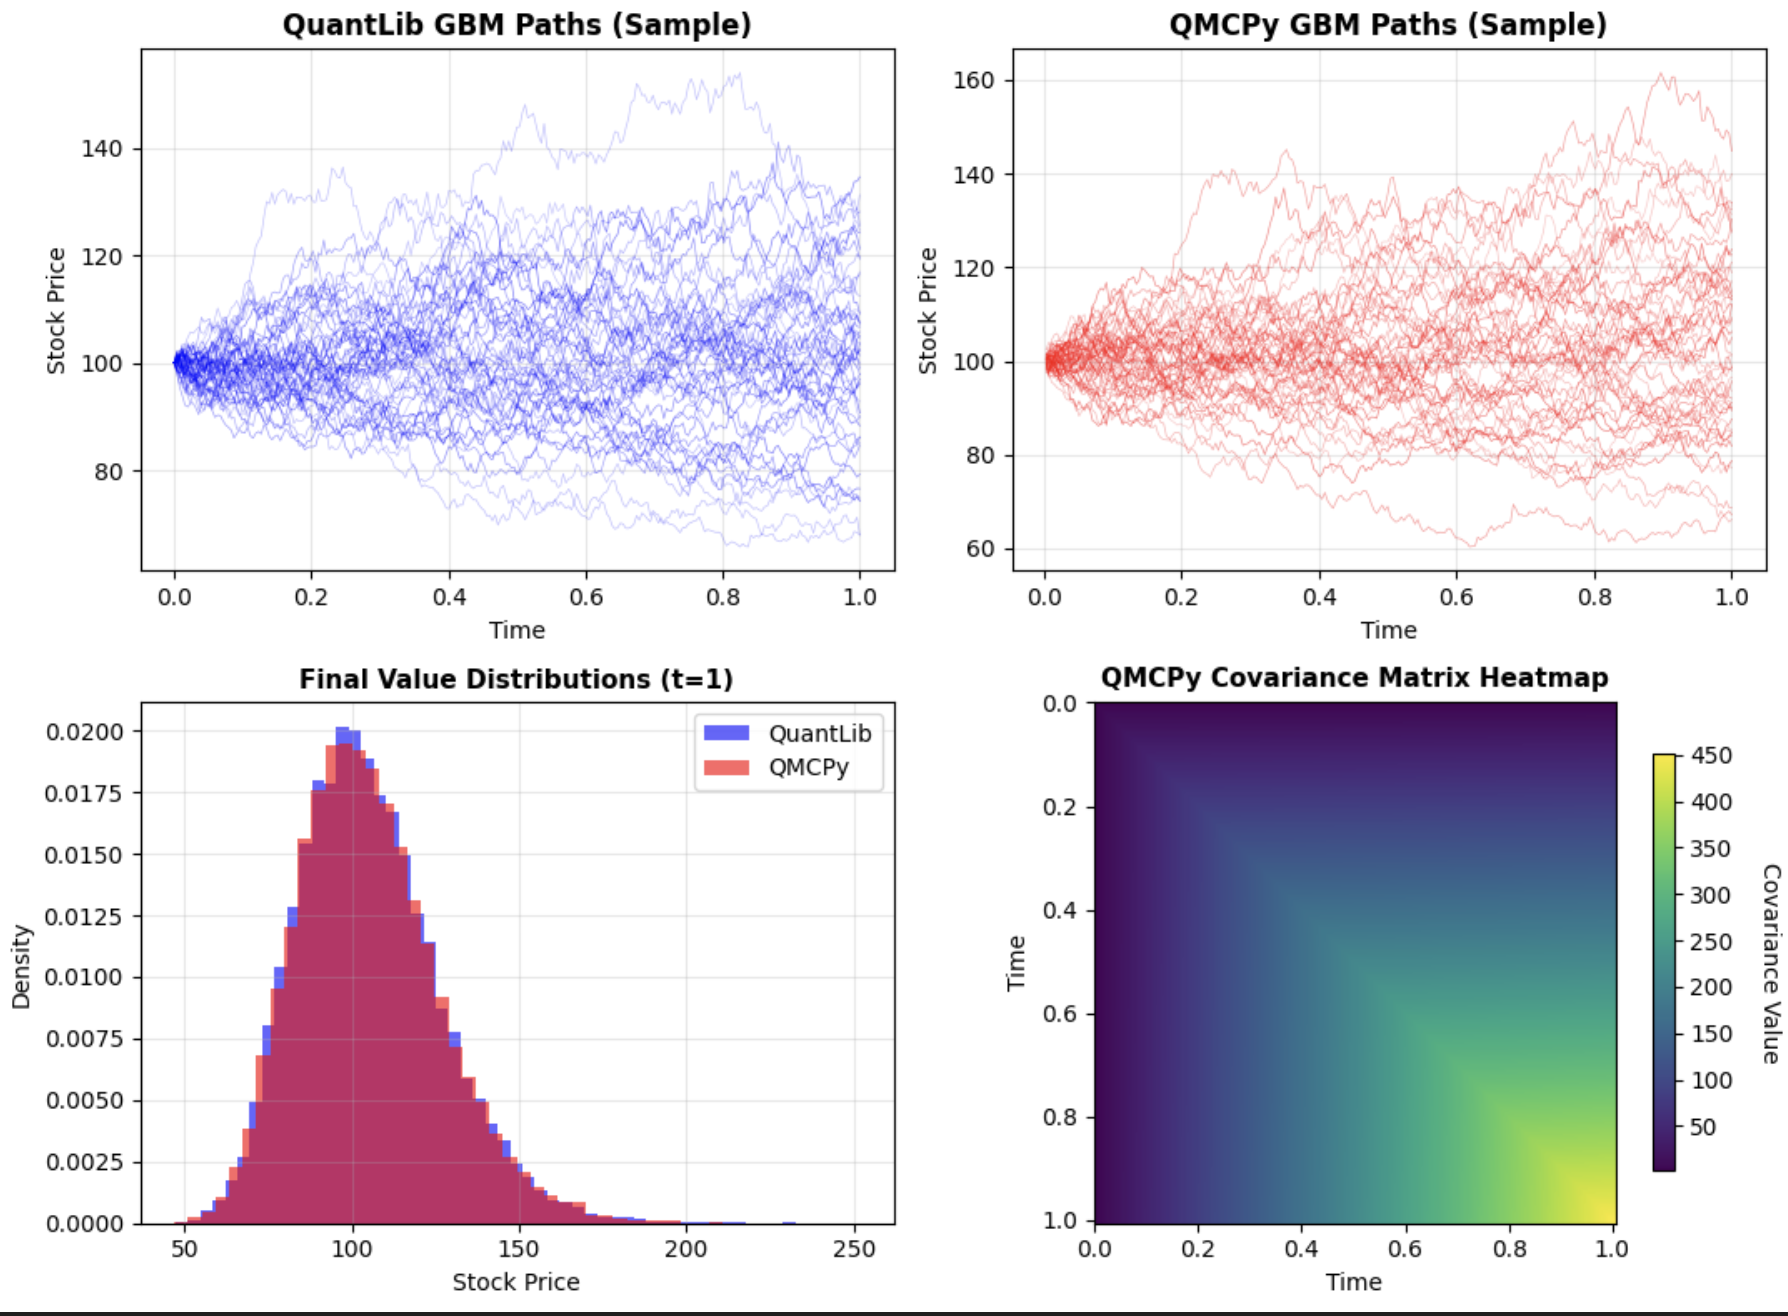
\includegraphics[width=1\textwidth]{GBM/images//figure_5.png}
\caption{QMCPy vs QuantLib comparison. Top: sample paths from QMCPy (left) and QuantLib (right). Bottom left: marginal distribution at $t=1$ showing close agreement between libraries and with Table~\ref{tab2}. Bottom right: QMCPy covariance heatmap (time 0 at top), consistent with the numerical matrix in Table~\ref{tab1}.}
\label{fig:qmcpy_quantlib_comparison}
\end{figure}

To evaluate computational efficiency, we conducted comprehensive performance benchmarks comparing QMCPy and QuantLib across two key scaling dimensions. The benchmarks were performed using the \texttt{perfplot} library, which automatically handles warm-up, multiple runs, and statistical analysis to ensure reliable timing measurements. 

Figure~\ref{fig:gbm_performance} presents the results of our performance analysis. The left panel (a) shows how execution time scales with the number of time steps while keeping the number of paths fixed at 4,096. Both libraries exhibit approximately linear scaling, but QMCPy demonstrates superior performance at smaller time step counts, with QuantLib becoming more competitive as the number of time steps increases. The right panel (b) examines scaling behavior with respect to the number of paths while fixing the time steps at 252 (representing a typical trading year). Here, QMCPy maintains a consistent performance advantage across all path counts, with the gap becoming more pronounced at higher path numbers. This performance difference is particularly relevant for Monte Carlo applications that require large numbers of simulation paths for accurate estimation.

\begin{figure}[H]
    \centering
    \begin{subfigure}{1\textwidth}
        \centering
        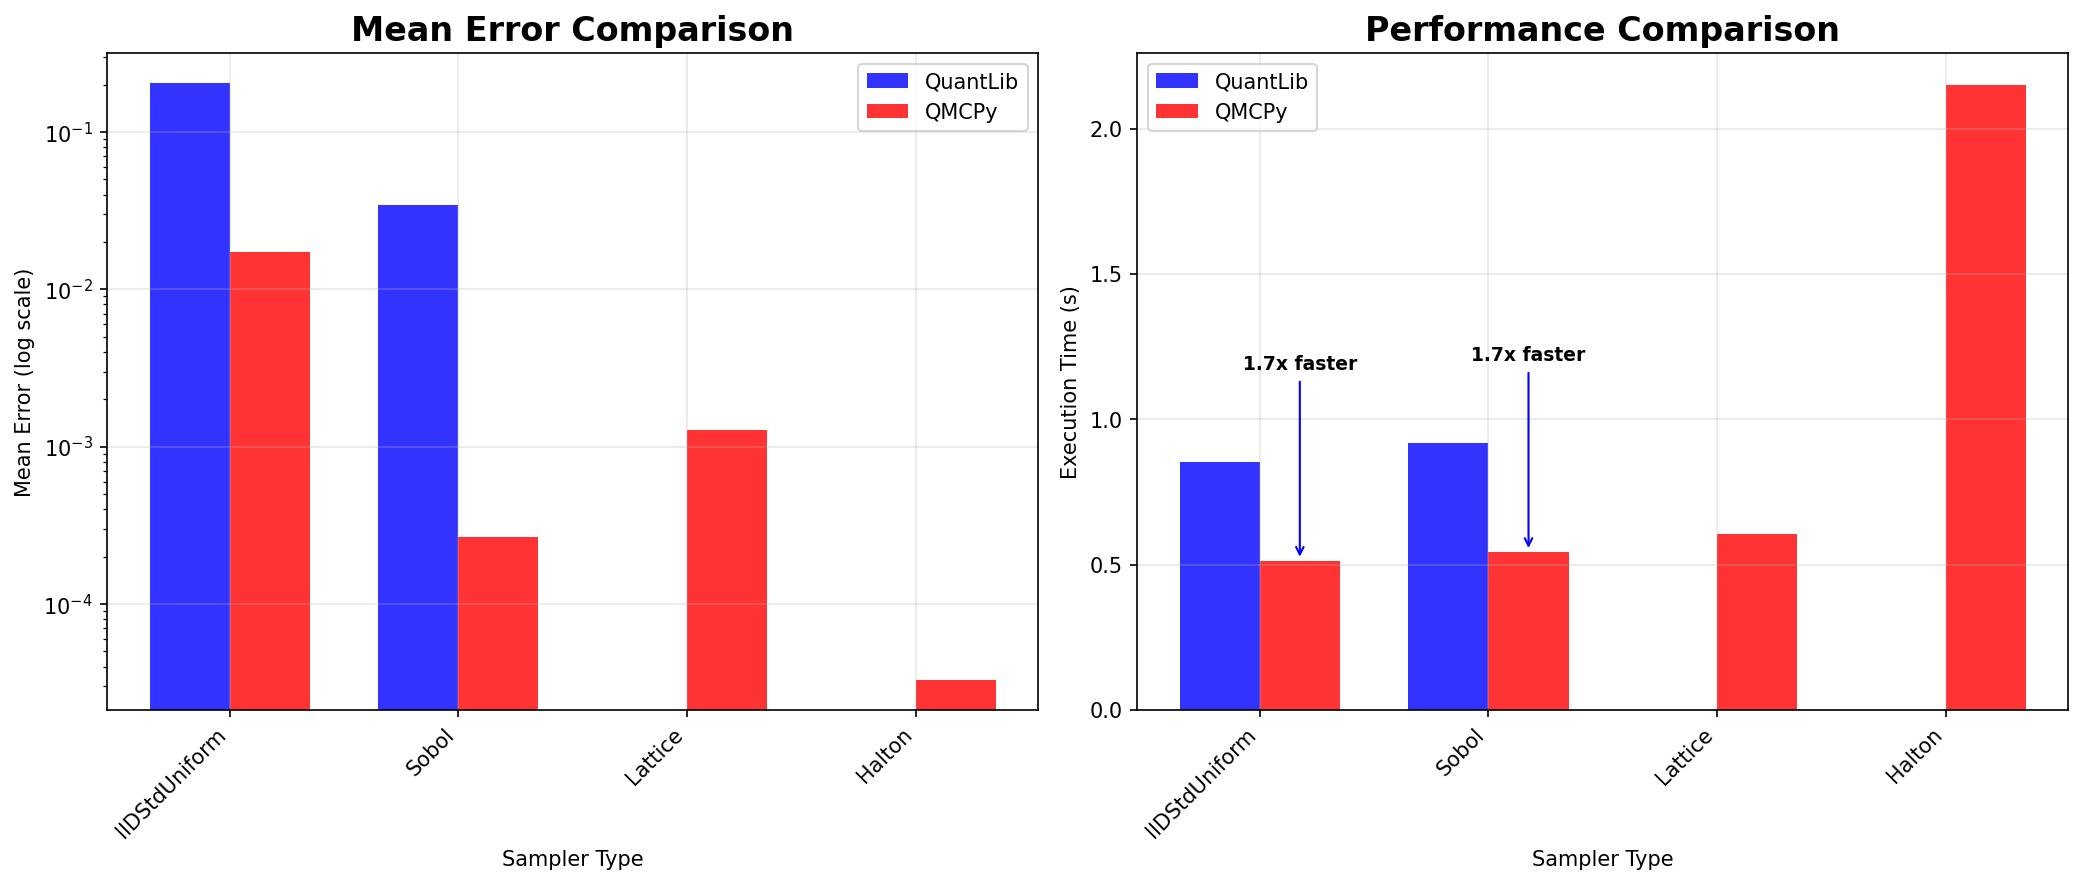
\includegraphics[width=\textwidth]{GBM/images//figure_6.png}
        %\caption{Performance vs Number of Time Steps}
        %\label{subfig:performance}
    \end{subfigure}
    %\hfill
    \caption{GBM Performance Comparison: QuantLib vs QMCPy. Left plot shows performance scaling with number of time steps for fixed paths. Right plot shows performance scaling with number of paths for fixed number of time steps.}
    \label{fig:gbm_performance}
\end{figure}

To further validate these performance findings, we conducted an extended parameter sweep analysis across a broader range of configurations. Figure~\ref{fig:gbm_performance2} presents the comprehensive results of this analysis, systematically examining performance across varying time steps and path counts. The extended benchmarks confirm QMCPy's consistent computational advantages and demonstrate robust scaling behavior across the parameter space, reinforcing its suitability for high-performance quasi-Monte Carlo applications.

\begin{figure}[H]
    \centering
    \begin{subfigure}{1\textwidth}
        \centering
        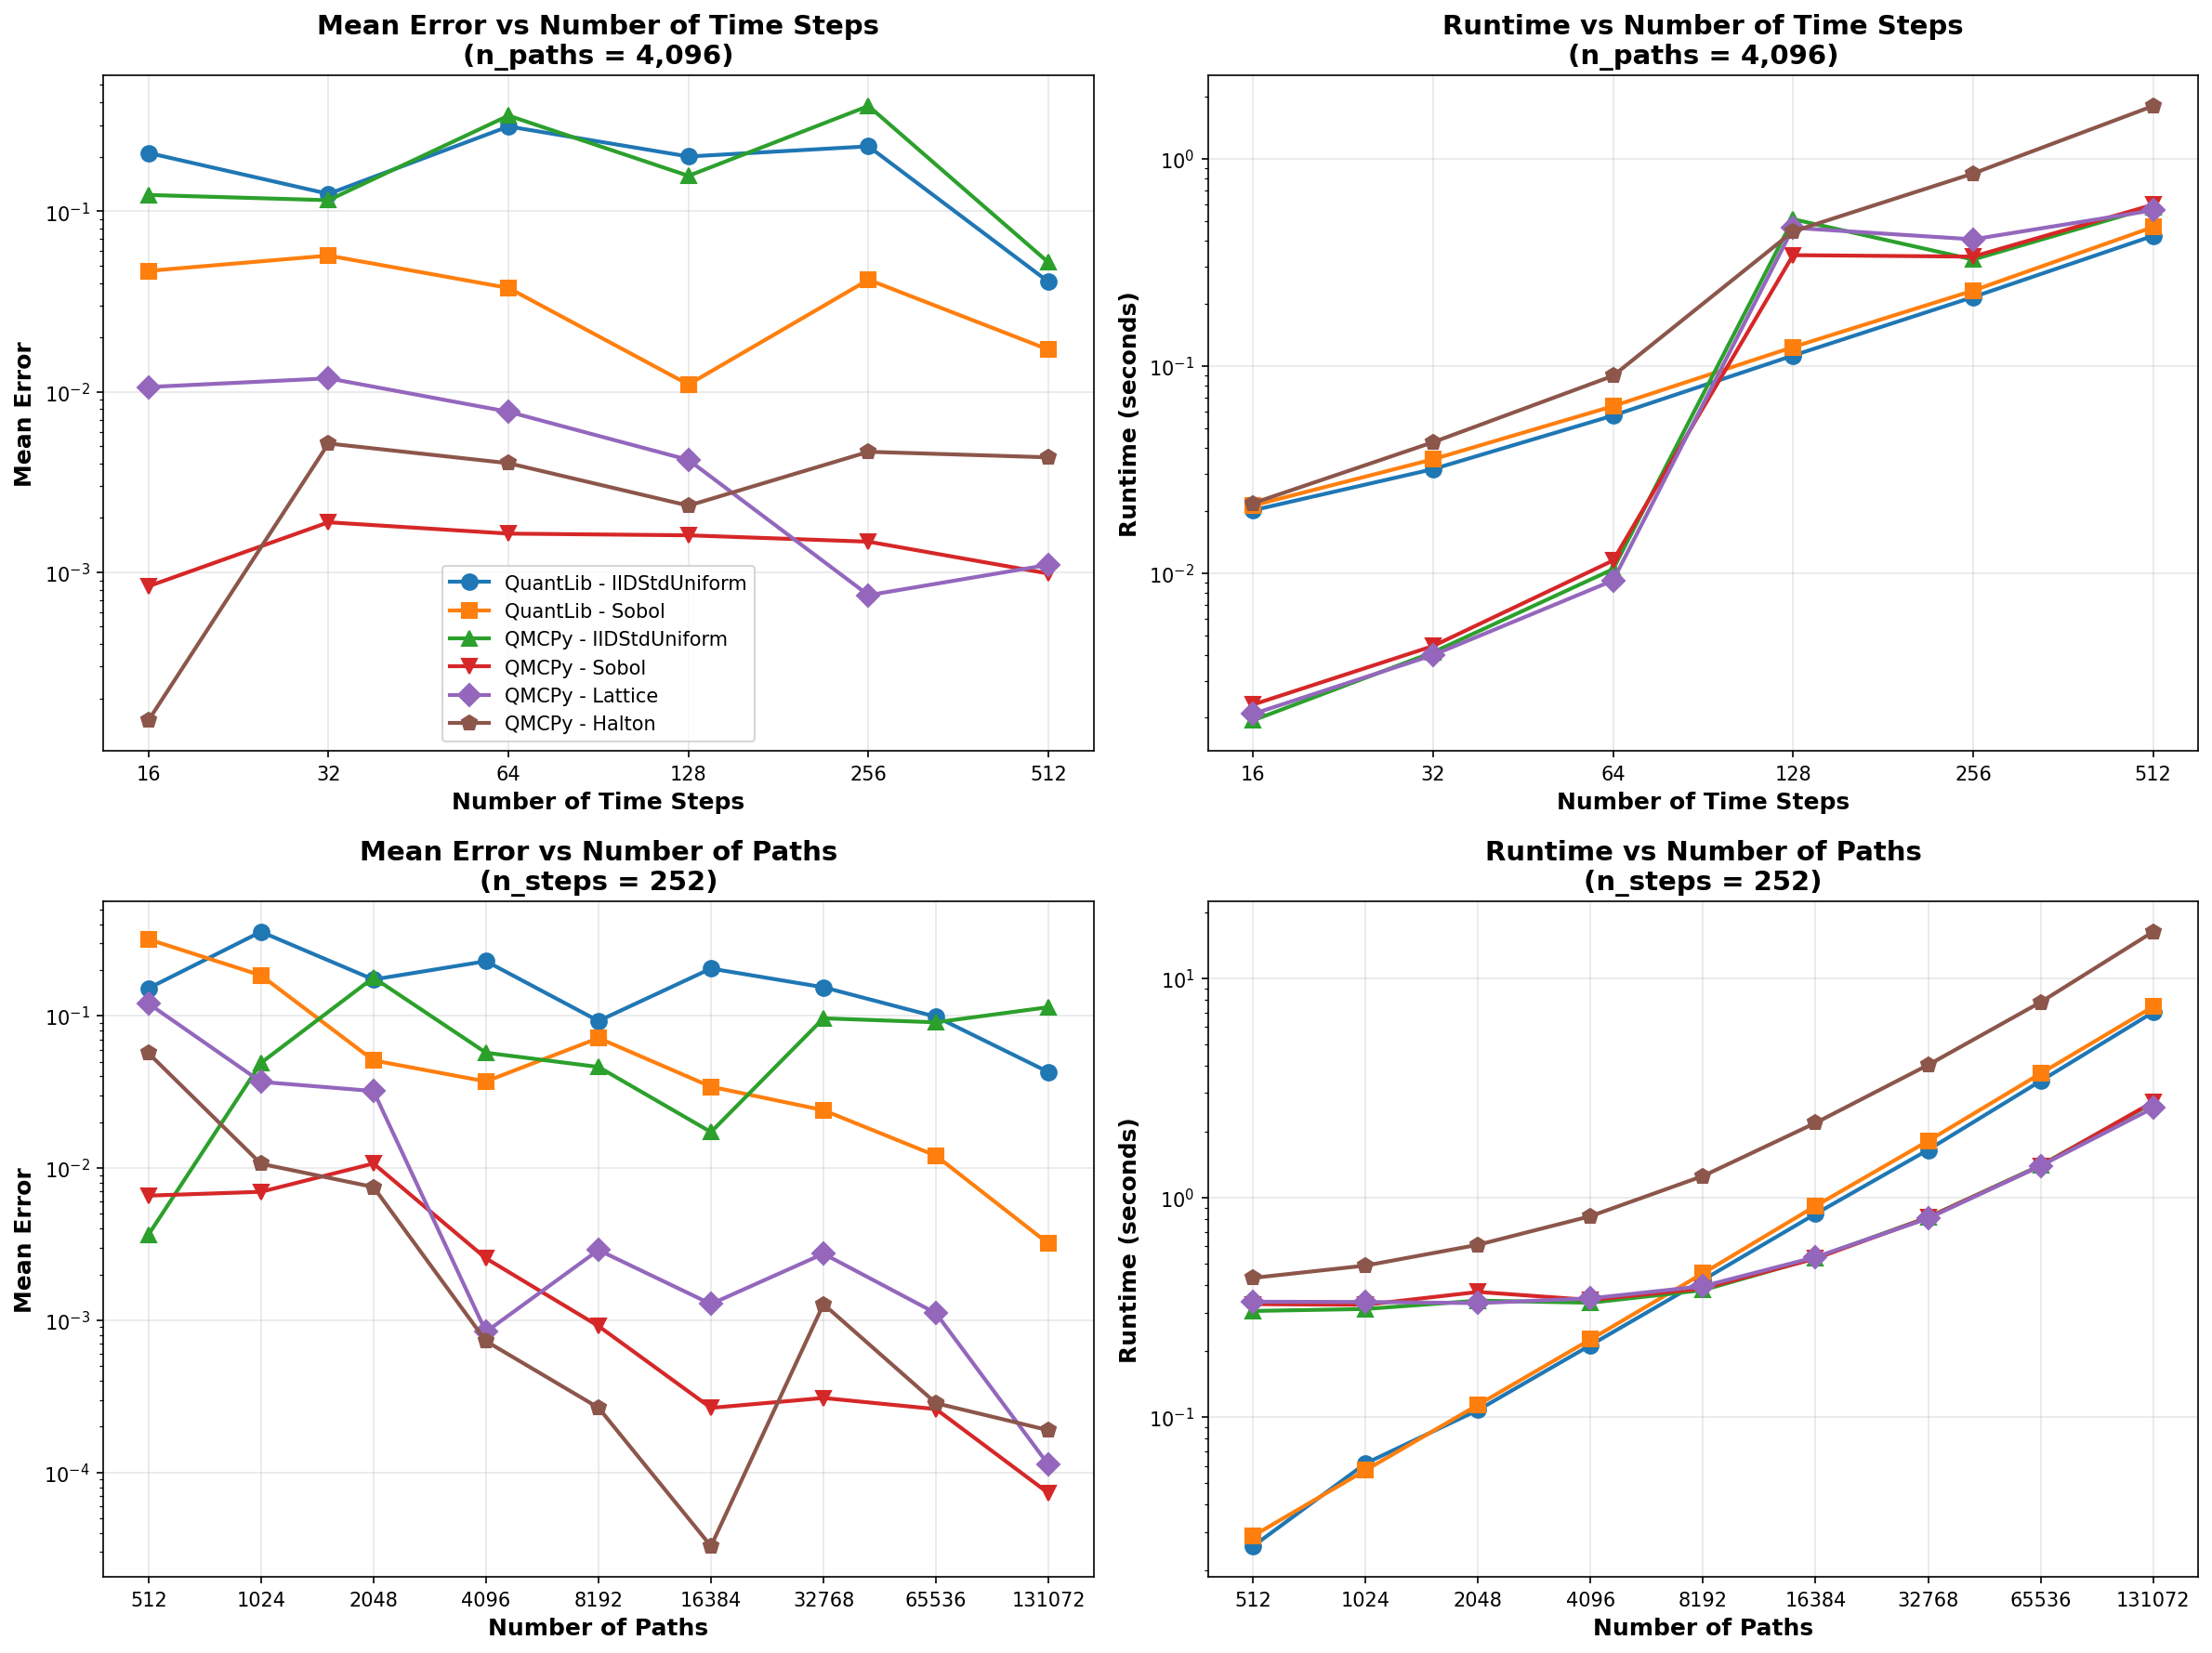
\includegraphics[width=\textwidth]{GBM/images//figure_7.png}
        %\caption{Performance vs Number of Time Steps}
        \label{subfig:performance_steps2}
    \end{subfigure}
    \begin{comment}
    \end{comment}
    \caption{Comprehensive parameter sweep performance analysis comparing QuantLib and QMCPy across varying time steps and path counts. The results demonstrate QMCPy's consistent performance advantages and superior scaling characteristics for both dimensions of the parameter space.}
    \label{fig:gbm_performance2}
\end{figure}

\subsection{Internals}

The \texttt{GeometricBrownianMotion} class in QMCPy is engineered for speed, robustness, and mathematical correctness. Its design leverages object-oriented inheritance and vectorized operations, resulting in both flexibility and high performance.
\texttt{GeometricBrownianMotion} inherits from \texttt{BrownianMotion} which itself inherits from \texttt{Gaussian}. This layered design allows the GBM class to reuse and extend efficient implementations for Gaussian random vectors and BM increments.
The constructor rigorously checks input parameters (e.g., positivity of initial value and diffusion, valid decomposition type), ensuring mathematical integrity and preventing run-time errors.

The class uses vectorized NumPy operations to generate entire arrays of GBM paths in a single call, minimizing Python loops and maximizing computational throughput. Sample generation proceeds in two stages:
\begin{enumerate}
\item 
The parent class \texttt{BrownianMotion} generates standard BM sample paths using the specified sampler (e.g., low-discrepancy lattice, IID uniform), with drift and diffusion handled in the mean and covariance structure.
\item  The GBM class transforms the BM samples via the exponential mapping \eqref{gbm}, performed in a fully vectorized fashion, ensuring that thousands of paths can be efficiently simulated.
\end{enumerate}
The class computes and stores the theoretical mean and covariance matrices for GBM at initialization, which can be used for validation and theoretical comparisons. Both mean and covariance are calculated using analytical formulas, leveraging \href{https://numpy.org/devdocs/user/basics.broadcasting.html}{NumPy’s broadcasting} for efficient computations. (Briefly, broadcasting in NumPy allows arithmetic operations between arrays of different shapes by automatically expanding the smaller array to match the shape of the larger array.)

 The Gaussian and BM classes both implement Cholesky and PCA factorization of the covariance matrix
\[
\Sigma \;=\; L\,L^{\!\top}
\quad\text{and}\quad
\Sigma \;=\; P\,D\,P^{\!\top},
\]
respectively.  In the Cholesky method, one computes the lower‐triangular $L=\operatorname{chol}(\Sigma)$ and obtains correlated increments via $X=L\,Z$, where $Z\sim\mathcal{N}(0,I)$.  In the PCA approach, one first diagonalizes $\Sigma=PDP^{\!\top}$, then forms $X = P\,D^{1/2}\,Z$.  By default PCA is used for its superior numerical stability in high dimensions and slightly lower cost when many eigenvalues are near zero.  These correlated normals feed directly into the GBM update
\[
S_{t+\Delta t} \;=\; S_t\,\exp\!\Bigl((\mu - \tfrac12\sigma^2)\Delta t \;+\;\sigma\sqrt{\Delta t}\,X\Bigr),
\]
ensuring that the simulated paths respect the intended covariance structure and remain strictly positive (with strict‐positivity checks raising warnings or errors if violated).

\bigskip
\begin{tcolorbox}[title=Takeaways,colback=blue!1,colframe=blue!30!black]
To the best of our knowledge, this blog presents the first publicly available benchmark comparing QuantLib and QMCPy for Geometric Brownian Motion (GBM) simulations. Key takeaways include:
\begin{itemize}%[topsep=0pt,itemsep=0pt,parsep=0pt,leftmargin=*]
    \item Flexibility: Change one argument in QMCPy to swap samplers or covariance decompositions.
    \item Accuracy: QMCPy's GBM matches QuantLib and theoretical moments, with superior numerical accuracy for quasi-Monte Carlo samplers (see Table~\ref{tab2}).
    \item Speed: Vectorized operations and optimized memory management produce 1.5 to 2 times faster path generation in QMCPy than QuantLib.
\end{itemize}
\end{tcolorbox}


\begin{thebibliography}{6}

\bibitem[1]{glasserman2003}
Glasserman, P. (2003). \textit{Monte Carlo Methods in Financial Engineering}. Springer.

\bibitem[2]{choi2022}
Choi, S.-C. T., Hickernell, F. J., Jagadeeswaran, R., McCourt, M. J., \& Sorokin, A. G. (2022).
Quasi-Monte Carlo Software. In A. Keller (Ed.), \textit{Monte Carlo and Quasi-Monte Carlo Methods}.
Springer International Publishing. DOI: \url{https://doi.org/10.1007/978-3-030-98319-2_2}.

\bibitem[3]{qmcpy2023}
Choi, S.-C. T., Hickernell, F. J., Jagadeeswaran, R., McCourt, M. J., \& Sorokin, A. G. (2020--2025).
QMCPy: A quasi-Monte Carlo Python Library (Version 2.1).
DOI: \url{https://doi.org/10.5281/zenodo.16822646}. 
Retrieved from \url{https://www.qmcpy.org}.

\bibitem[4]{hull2017}
Hull, J. C. (2017). \textit{Options, Futures, and Other Derivatives} (10th ed.). Pearson.

\bibitem[5]{ross2014}
Ross, S. M. (2014). \textit{Introduction to Probability Models} (11th ed.). Academic Press.

\bibitem[6]{quantlib} 
The QuantLib contributors (2003--2025). 
QuantLib: A free/open-source library for quantitative finance (Version 1.38).
DOI: \url{https://doi.org/10.5281/zenodo.1440997}. 
Retrieved from \url{https://www.quantlib.org}.
% https://github.com/lballabio/QuantLib/commit/87c5ee2e17e9dd17488ec9957159b89db18d5d26
\end{thebibliography}